%%%%%%%%%%%%%%%%%%%%%%%%%%%%%%%%%%%%%%%%%
% University Assignment Title Page
% LaTeX Template
% Version 1.0 (27/12/12)
%
% This template has been downloaded from:
% http://www.LaTeXTemplates.com
%
% Original author:
% WikiBooks (http://en.wikibooks.org/wiki/LaTeX/Title_Creation)
%
% License:
% CC BY-NC-SA 3.0 (http://creativecommons.org/licenses/by-nc-sa/3.0/)
%

%%%%%%%%%%%%%%%%%%%%%%%%%%%%%%%%%%%%%%%%%
%\title{Title page with logo}
%----------------------------------------------------------------------------------------
% PACKAGES AND OTHER DOCUMENT CONFIGURATIONS
%----------------------------------------------------------------------------------------

\documentclass[paper=a4, fontsize=11pt]{scrartcl}
\linespread{1.25}
\usepackage[english]{babel}
\usepackage[utf8x]{inputenc}
\usepackage{mathtools}
\usepackage{graphicx}
\usepackage{booktabs}
\usepackage{cite}
\usepackage{textcomp}
\newcommand{\textapprox}{\raisebox{0.5ex}{\texttildelow}}
\usepackage[nottoc]{tocbibind}

\usepackage{listings}
\lstset{breaklines}
\setcounter{secnumdepth}{4}
\usepackage{tikz}
\usepackage{xfrac}
\usetikzlibrary{arrows.meta}
\tikzset{%
  >={Latex[width=2mm,length=2mm]},
  % Specifications for style of nodes:
            base/.style = {rectangle, rounded corners, draw=black,
                           minimum width=4cm, minimum height=1cm,
                           text centered, font=\sffamily}
}
\begin{document}

\begin{titlepage}

\newcommand{\HRule}{\rule{\linewidth}{0.5mm}} % Defines a new command for the horizontal lines, change thickness here

\center % Center everything on the page

%----------------------------------------------------------------------------------------
% HEADING SECTIONS
%----------------------------------------------------------------------------------------

\textsc{\LARGE EURECOM}\\[1.5cm] % Name of your university/college
%\textsc{\Large Major Heading}\\[0.5cm] % Major heading such as course name
%\textsc{\large Minor Heading}\\[0.5cm] % Minor heading such as course title

%----------------------------------------------------------------------------------------
% TITLE SECTION
%----------------------------------------------------------------------------------------

\HRule \\[0.4cm]
{ \huge \bfseries Music Recommendation when Exploring a City}\\[0.4cm] % Title of your document
\HRule \\[1.5cm]

%----------------------------------------------------------------------------------------
% AUTHOR SECTION
%----------------------------------------------------------------------------------------

\begin{minipage}{0.4\textwidth}
\begin{flushleft} \large
\emph{Authors:}\\
Lorenzo \textsc{Canale} % Your name
\newline
Fabio \textsc{Ellena} % Your name
\end{flushleft}
\end{minipage}
~
\begin{minipage}{0.4\textwidth}
\begin{flushright} \large
\emph{Supervisor:} \\
Pasquale \textsc{Lisena} \\ % Supervisor's Name
Raphaël  \textsc{Troncy} % Supervisor's Name
\end{flushright}
\end{minipage}\\[2cm]

% If you don't want a supervisor, uncomment the two lines below and remove the section above
%\Large \emph{Author:}\\
%John \textsc{Smith}\\[3cm] % Your name

%----------------------------------------------------------------------------------------
% DATE SECTION
%----------------------------------------------------------------------------------------

%{\large \today}\\[2cm] % Date, change the \today to a set date if you want to be precise

%----------------------------------------------------------------------------------------
% LOGO SECTION
%----------------------------------------------------------------------------------------

\includegraphics[scale=0.8]{images/logo.jpg}\\ % Include a department/university logo - this will require the graphicx package

%----------------------------------------------------------------------------------------

\vfill % Fill the rest of the page with whitespace

\end{titlepage}
\begin{abstract}
Abstract:
Our project aims at making the user discover the existing connections that link music to a Place, by stimulating his curiosity proposing non-common relations. In this project, we show a new approach for finding artists linked to a place of interest (POI). We propose an entity linking framework built on top of DBpedia, 3cixty, and DOREMUS that is able to reach editorial accuracy in the interlinking process. Furthermore, we present a graph exploration algorithm that is able to find deep connections in a short time and discriminate between them by looking at those that can be the most interesting.
\end{abstract}
\newpage

\tableofcontents
\newpage

\section{Introduction}
"In order to generate relevant recommendations, a context-aware recommender system (CARS) not only makes use of user preferences, but also exploits information about the specific contextual situation in which the recommended item will be consumed."~\cite{Baltrunas:2012:CRA:2339097.2339111}

This is in contrast with the fact that most of the available music recommender systems suggest music without taking into consideration the user context~\cite{Knees:2013:SMS:2559928.2542206}. This is because defining and especially exploiting contexts is not a trivial operation. Context can be defined as any information that can be used to characterize the situation of an entity~\cite{Dey:2001:UUC:593570.593572}. These information information includes mood, location, activity, friends, daily and current activities of the target user.

If we think of a recommender task in a mobile scenario (e.g., choosing a song while sightseeing), we see that most recommendations are requested by users while they are on their way. This causes a continuous change in the context that needs to be carefully addressed. Recommendations are much more useful and enjoyable for end users as they change with their current context~\cite{Ostuni:2012:CCM:2887638.2887642}.

Finding music that suits a Point of Interest(POIS) can be viewed as a context-aware recommendation problem, the place is the context for consuming the recommendation. The main challenge that one must face when addressing the above-mentioned goal is related to the fact that POIs and music are two rather different domains, and there is no obvious way to match such heterogeneous items. However, with the advent of the Semantic Web, new opportunities arise to face these type of difficulties. We will show that, using a general purpose semantic dataset such as DBpedia, we can recommend artists that are linked to the user location.

\subsection{Motivation and context}
In the past, different attempts have been performed to link POIs and music in many different ways. A strategy can consist in linking music and POIs by using a common set of tags that describe emotional properties both for music and POIs~\cite{Kaminskas:2013:LMR:2507157.2507180}. This method is completely supervised, in fact it requires the definition of a set of emotions for songs and POIs. This operation must be done manually and is hardly scalable.
\begin{figure}[!htb]
  \centering
    \includegraphics[width=1\textwidth]{images/semantic_net.png}
    \caption{Semantic Network with predefined classes}
\end{figure}

In~\cite{Kaminskas:2012:KMR:2390848.2390854}, the goal is achieved by by restricting the subspace of DBpedia to a set classes related to the domains of interest. These classes includes concepts that are easily linkable to artists and POIs, such as historic periods, architectural styles and geographic information. In this way, it is possible to find relations in a set of paths constrained to pass through those classes.
Looking at the future propositions, both strategies proposed the idea to exploit arbitrary semantic relations between POIs and musicians.
In order to do this, tools like Relfinder have been proposed \cite{Heim:2009:RRR:1695324.1695351}, in combination an heuristic to set the connection weights. In fact, one of the disadvantages of those approaches is that connections weights are assigned by experts and are not published.
Our goal is to build our approach on top of this paper and find relations in a completely unsupervised way: this means that we intend to define a path finder that finds paths and a path discriminator that selects the interesting relations.

\subsection{Research problems}
The main challenge is the goal itself: is it possible to suggest interesting artists based on the user context?
Since we intend to find DBpedia relations between POIs and artists, how deep are this kind of relations? Are there tools that have already solved completely this problem? In which context they work and are they scalable on a big number of entities? What is the shape of these connections? Do they have a common pattern? How many are they? Can we filter only the interesting ones? How can we define an interesting connection?

It is our intention to use specialized datasets that are not directly linked to DBpedia. Therefore, What are the important properties to consider when doing such a job?

\subsection{Contributions}
In this project, we show a new approach for finding artists linked to a place of interest (POI). We propose an entity linking framework built upon DBpedia, 3cixty\footnote{3cixty: https://www.3cixty.com/}, and DOREMUS\footnote{DOREMUS: http://www.doremus.org/} that is able to reach editorial accuracy in the interlinking process. Furthermore, we present a graph exploration algorithm that is able to find deep connections in a short time and discriminate between them by looking at those that can be the most interesting.
We aim at reducing the need for human intervention in defining classes and weights with the hope that this approach will be completely data driven and easily scalable to different cities.
Finally, we demonstrate the effectiveness of our work through an APP that drives the user experience in the exploration of a city, recommending songs linked to the user position. In addition it presents the reason of the recommendation through a graphical visualization of the path between the artist that composed the song and the POI chosen for the recommendation.
For this experimental work, we chose Nice because because it is a medium sized city that allows us to deal with both popular and unpopular places. Furthermore the number of POIs in Nice is manageable, this means that we can check immediately our results. Finally, POIs in Nice are enough to see if our proposed solution can scale.

\subsection{Report structure}
This report is divided into five sections, one for each part of the project. The first two parts are about linking external datasets to DBpedia, this task is known as entity linking and we perform it in the optic of enriching our data with the inter-concept links present in DBpedia.
The third covers the Pathfinder, a module of our system that is able to find deep connections between two entities in DBpedia.
The fourth describes the whole implementation of the REST API that allows the application to work smoothly.
The fifth part covers the mobile web application and the technologies involved in its functioning.

\section{Interlinking and enriching POIs}
\subsection{Problem description}
Interlinking different datasets is not trivial, many approaches that aimed at a semi-supervised interlinking have been proposed, but this is still an active research topic.
One of the main problems that must be faced in an interlinking process is the ontology definition. In fact, specialized datasets tend to have a very strict ontology, while DBpedia does not enforce it. This means that in the case of POIs, not all places in Nice are linked to Nice, thus it is difficult to even correctly define a POI in Nice.
Since we are dealing with a medium sized city such as Nice, we can't allow loosing some matchings and we need to carefully analyze the DBpedia ontology in order to leave out the minimum part of Nice POIs.

\subsection{Datasets: 3cixty, DBpedia, Wikidata}
\subsubsection{3cixty}
3cixty is a semantic dataset that contains aggregated information of POIs and events. The dataset is the result of an aggregation process that join the POI information from different datasets e.g. Facebook, Foursquare, Yelp \dots
In this project 3cixty is used as a trusted source of POIs for Nice.
POIs have a lot of information, such as the category, the address, comments from users, and coordinates. In order to get all the POIs in Nice, we simply used the POIs endpoint of the 3cixty API.

For example, this is the JSON object associated to the `Nice Lawn Tennis Club': \begin{lstlisting}
{
   "_about":"http://data.linkedevents.org/location/579aa423-cb1b-3d35-90d5-ef482aa093ad",
   "businessType":[
      "http://data.linkedevents.org/kos/foursquare/tennis-court"
   ],
   "geoLocation":{
      "_about":"http://data.linkedevents.org/location/579aa423-cb1b-3d35-90d5-ef482aa093ad/geometry",
      "lat":43.7043,
      "long":7.25188
   },
   "label":"Nice Lawn Tennis Club",
   "location":{
      "_about":"http://data.linkedevents.org/location/579aa423-cb1b-3d35-90d5-ef482aa093ad/address",
      "streetAddress":"5, ave. Suzanne Lenglen, 06000 Nice, France"
   }
}

\end{lstlisting}
\subsubsection{DBpedia}
DBpedia\footnote{DBpedia: http://wiki.dbpedia.org/} is a crowd-sourced community effort to extract structured information from Wikipedia\footnote{Wikidata: https://en.wikipedia.org/} and make this information available on the Web. The DBpedia knowledge base has several advantages over existing knowledge bases: it covers many domains; it automatically evolves as Wikipedia changes, and it is truly multilingual.
We used it to get the POIs in Nice.
In order to get the POIs from DBpedia, it is necessary to perform SPARQL queries against the SPARQL endpoint. POIs are retrieved using two different SPARQL queries that target different kind of resources:
\begin{enumerate}
\item We perform a query that looks for all resources in Nice.
Figure \ref{fig:box} shows the area with valid coordinates.
Unfortunately there are many POIs that are without coordinates, so they are not selected by this query.
\begin{lstlisting}
SELECT ?place ?placeLabel ?lat ?long
WHERE {
    ?place geo:lat ?lat.
    ?place geo:long ?long.
    ?place rdfs:label ?placeLabel.
    FILTER(
      xsd:double(?lat)  <= 43.80 &&
      xsd:double(?lat) >= 43.63 &&
      xsd:double(?long) <= 7.36 &&
      xsd:double(?long) >= 7.14
    )
}
\end{lstlisting}
\begin{figure}[!htb]
  \centering
    \includegraphics[width=0.5\textwidth]{images/Nice.png}
    \caption{Area for POIs selection}
    \label{fig:box}
\end{figure}

\item We take all resources that have as a parent either the dbr:Nice resource or the dbc:Nice resource. Then we repeat this operation for each subcategory of dbc:Nice in a recursive way. Among these resources, we keep those which type is in a set of classes defined by hand.
\end{enumerate}
\subsubsection{Wikidata}
Wikidata\footnote{Wikidata: https://www.wikidata.org/} Wikidata is a free and open knowledge base that can be read and edited by both humans and machines. Wikidata acts as central storage for the structured data of its Wikimedia\footnote{Wikimedia: https://www.wikimedia.org/} sister projects including Wikipedia.

We used it to get the POIs in Nice. Respect to DBpedia, Wikidata has a well defined ontology that is strictly enforced. This means that it is easier to select what we want. Moreover, most of POIs in wikidata have coordinates, so we can get them with a single query. Since wikidata supports complex geo-based queries, we can make a query that looks for all POIs in a range of 25 Kilometers from the center of Nice.
\begin{lstlisting}
SELECT ?item ?itemLabel ?location WHERE {
  wd:Q33959 wdt:P625 ?niceLoc .
  SERVICE wikibase:label {
    bd:serviceParam wikibase:language "fr" .
  }.
  SERVICE wikibase:around {
      ?item wdt:P625 ?location .
      bd:serviceParam wikibase:center ?niceLoc .
      bd:serviceParam wikibase:radius "10" .
  }
}
\end{lstlisting}

\subsection{Entity Linking process}

\begin{figure}[!htb]
  \centering
    \includegraphics[width=1\textwidth]{images/pipeline.png}
    \caption{Entity linking pipeline}
    \label{fig:pipeline}
\end{figure}


Figure \ref{fig:pipeline} summarizes the main steps, datasets, and outputs of the entity linking process.
In order to link our three set, we copy them locally and then we perform the linking process. Having the entities locally is crucial, in fact it allows us to make way more complex operations respect to those that can be done with SPARQL queries. The whole process can be described as follow:
\begin{enumerate}
\item Extract labels from DBpedia entities.
\item Apply transformations.
\item Compute similarity metrics with 3cixty entities.
\item Aggregate results
\item Filter matches above threshold.
\item Evaluate results.
\end{enumerate}

\subsubsection{Properties}
The first phase is to actually get the interesting properties of the entities. Regarding those that come from DBpedia, we use only the labels. Regarding the labels, we take them in all the available languages. In this way we can do a multilingual match that improves our accuracy.
Here is an example:
\begin{itemize}
\item DBpedia labels: `Conservatory of Nice' @en, `Conservatoire de Nice' @fr
\item 3cixty label: `Conservatoire de Nice'
\end{itemize}
In this case if we use the English label, we do not obtain a perfect match, while with the French label we obtain a perfect match. Other times we have the opposite result, but using labels in different languages we solve this problem.

\begin{figure}[!htb]
  \centering
    \includegraphics[width=0.5\textwidth]{images/parc.png}
    \caption{Parc Phœnix coordinates: blue marker from DBpedia, red marker from Google Maps}
    \label{fig:parc}
\end{figure}

Among other information, we have the coordinates, but we do not use them because not all entities have them. Moreover, we have seen experimentally that using the DBpedia coordinates we obtain worse results because of their inaccuracy. This is clearly visible in Figure~\ref{fig:parc}.
Regarding 3cixty entities, they have very accurate coordinates and few labels. For this phase we do not need the coordinates, while regarding the labels, we keep the first one.

\subsubsection{Transformations}
At this point of the pipeline, we have labels that are encoded into unicode utf-8. Common similarity metrics accepts only plain ASCII strings as input, so we need to convert them into ASCII. Since utf-8 can represent way more characters than ASCII, we need to strip non ASCII characters from our labels. This is done in an intelligent way using the python library \textit{`unidecode'}\footnote{Unidecode: https://pypi.python.org/pypi/Unidecode}, that is able to convert from unicode to ASCII by changing or deleting a minimum set of characters. For example, an accented letter like `è' can't be represented in ASCII, and most of the libraries simply delete it, while \textit{`unidecode'} converts it to the nearest ASCII character: in this case 'è' is converted to 'e'. In this way we can retain most of the original information after this conversion process.

The second step is probably the most important, and is the normalization of names. Some similarity metrics are extremely sensitive to noise. For example, when we use simple Levenshtein:
\begin{itemize}
\item levenshtein\_distance(`airport',`airport nice'): 5
\item levenshtein\_distance(`airport',`port'): 4
\end{itemize}
This is enough to raise some concerns: the simple addition of the city name can turn a perfect match into a mediocre one. In order to fix this problem we add the city name to all the labels where it is not present.

The third step is to strip all non alphabetical characters and to convert to lowercase all strings, this off course gives us cleaner strings to compare.

The whole transformation pipeline aims at maximizing the similarity measure between correct matches. Later we will set a threshold to separate matches that have a good confidence from matches with a low confidence.

\subsubsection{Similarity measures and matching algorithm}
Now that strings are clean, we can continue to the actual matching. A first question rises: we want to match a 3cixty poi to a DBpedia poi, or we want to match a DBpedia poi to a 3cixty poi? In the first case we are sure that each 3cixty poi will be matched to a single DBpedia poi, but there is the risk that multiple 3cixty poi are matched to the same DBpedia poi. Alternatively, we are sure that each DBpedia poi is matched to at most a 3cixty poi, but there is the risk that many DBpedia poi are matched to the same 3cixty poi.
Regarding DBpedia, we are sure that POIs are univoque, while we know that for the same POI, in 3cixty there are multiple ones.
Since at the end we will be using 3cixty coordinates, we opt for the first choice: if a DBpedia poi will be matched to multiple 3cixty pois, than we will follow an heuristic to choose the best match.

Regarding the similarity metric among strings, we use multiple similarity measures based on Levenshtein distance. This comes from the fact that experimentally we have seen experimentally that in this specific case, strings that represents POIs, a single similarity metric is not enough. From a technical point of view, we used a set of the similarity metrics provided by the `fuzzywuzzy'\footnote{FuzzyWuzzy: https://pypi.python.org/pypi/fuzzywuzzy} python module:
\begin{itemize}
\item partial\_ratio: Return the ratio of the most similar substring
    as a number between 0 and 100.
\item token\_set\_ratio: Find all alphanumeric tokens in each string:
\begin{enumerate}
\item treat them as a set
\item construct two strings of the form: $<sorted\_intersection> <sorted\_remainder>$
\item take ratios of those two strings
\item controls for unordered partial matches
\end{enumerate}

\item token\_sort\_ratio: Return a measure of the sequences' similarity between 0 and 100
    but sorting the token before comparing.
\item partial\_token\_sort\_ratio: Return the ratio of the most similar substring as a number between 0 and 100 but sorting the token before comparing.

\item WRatio: A weighted combination of other similarities
\end{itemize}

\subsubsection{Aggregations}
Until now, we took one by one the 3cixty labels and we calculated the different similarity metrics against all DBpedia labels.
The aggregation algorithm is run for each 3cixty POI and can be described as follow:
\begin{enumerate}
\item For each similarity metric, take the three best matching labels and for each of them, calculate the average of all the similarity metrics.
\item The final match is the POI corresponding with the label with the highest score.
\end{enumerate}
Why we don't simply take the average, or the minimum, or the maximum?
The reason behind this is that by taking the average we are flattening all the scores, and there is the risk that the string with the highest similarity is a string that is mediocre in all the different metrics. If a string is mediocre in all comparisons, then we do not trust it. Instead, with our methodology we are keeping only those matches that excel in some similarity metric, and then we take the one that performs better on average. In this way we can filter out all those matches with average strings that matches almost anything.

\subsubsection{Filtering}
Now that the matching is done, we need to filter our results.
The first operation to do is to ignore all those POIs that match with Nice, but that have a label different from Nice. This happens because we added Nice to all the strings. That addition was helpful, and it also created a safe default that we can easily filter.
Most of the POIs filtered in this way are acronyms that match with Nice, e.g. `ATP Nice' matches with Nice because half of the string is Nice and is artificial, because we added it.

The second operation to perform is the filtering based on the average score.
The average score can be interpreted as a confidence. Intuitively, high scores corresponds to correct matches, while low scores corresponds to bad matches.
The importance of the selection, transformation, similarity metric and aggregation pipeline is extremely high, in fact we want a confidence which we can trust. An untrusted confidence gives us no additional information about good matches and bad matches.
At this point we filter all matches with a score below a given threshold(0.8).

In this moment for each 3cixty POI we have a link to a DBpedia POI, but we might have multiple 3cixty POIs linked to the same DBpedia POI. We aim to a 1 to 1 relation, so we need to choose one among a group of 3cixty POIs linked to the same DBpedia POI, the most representative.
We have few possibilities:
\begin{enumerate}
\item Pick the POI that minimize the distance to all the other POIs, this is like applying the K-medoids clustering with K equal 1. This works if POIs are actually clustered, while it does not work if they are sparse.
\item Pick the POI which is nearest to the center. This is biased towards POIs near the center.
\item Pick the POI which is nearest to the DBpedia POI, if coordinates are available. This works only with a subset of POIs, and we do not fully rely on DBpedia coordinates.
\item Pick the POI which is nearest to the position found on Google Maps\footnote{Google Maps: https://www.google.fr/maps}. We have no control over Google Maps.
\item Link our data to GeoNames\footnote{GeoNames: http://www.geonames.org/}. Not all DBpedia POIs have a corresponding GeoNames POI.
\end{enumerate}
For simplicity and reliability, we used the Google Maps API because we trust it.
We use the API by sending the DBpedia label to the service, the response contains the coordinates of the POI associated to the DBpedia label. At this point we select the nearest 3cixty POI and we keep it if the distance is less than 2 kilometers.
\subsection{Evaluation (Google Maps)}
The evaluation part is done using the Google Maps API. As done before, we use the distance between the 3cixty POI coordinates and the POI coordinates provided by the API. Since we used the Google Maps API during our process, we expect that distances are low, in fact we know that each POI distance is less than 2 kilometers. What we want to check here is the distance distribution.

\begin{figure}[!htb]
  \centering
    \includegraphics[width=0.5\textwidth]{images/distance.png}
    \caption{distance distribution of POIs}
    \label{fig:poidist}
\end{figure}

Figure \ref{fig:box} shows the POIs distance distribution with the corresponding Google Maps POIs. If we consider 250 meters as a threshold, 70\% of POIs are below it. The main reason for this is the inherent error that arise when we define a POI which occupies a big surface with coordinates that refer to a specific point. For example the surface of the airport of Nice is quite big and different services can locate it in different points of his surface. In the case of the airport, the distance is actually 500 meters. This means that if it is true that most of the POIs are under 250 meters, we can't use this as a threshold because we would leave out a large part of the correct POIs.
At the end of our POI linking process we have 58 POIs.

\section{Interlinking and enriching Artists}
\subsection{Problem description}
DBpedia Artists and Works are not represented with a strict ontology.
This is a huge limit because we can not rely entirely on the data that we have in DBpedia. Even the simpler operations, such as finding all artists and all songs are extremely difficult due to the non-strict ontology of DBpedia. In order to have some order, we use DOREMUS, which contains trusted and properly organized information about artists and songs.

\subsection{Datasets: DOREMUS, DBpedia, Wikidata}
\subsubsection{DOREMUS}
DOREMUS is a semantic dataset that aims to a fine description of musical works in the fields of traditional and classical music: related musical or creation events, relations to authors, cultural background, interpretations, social functions, etc.
With DOREMUS we can have absolute trust in the data regarding artists, and we can then found corresponding artists in DBpedia with a custom linking process.
Retrieving all artists from DOREMUS is extremely easy, in fact we just need to ask for the Persons in the datasets that are linked to a work at least. The performed query is written below; we retrieved not only the artist uri but also the artist name, the id, the born year, the death year and the DBpedia `sameAs' link. These information are useful as input data for our similarity metric and for the final evaluation.

\begin{lstlisting}
SELECT $uri_doremus
(group_concat( distinct $id_doremus;separator="|||") as $id_doremus)
(group_concat(distinct $name_doremus;separator="|||") as $name_doremus)
(group_concat(distinct $born_year;separator="|||") as $born_year)
(group_concat( distinct $death_year;separator="|||") as $death_year)
(group_concat(distinct $dbpedia;separator="|||") as $dbpedia)
WHERE {
  $uri_doremus foaf:name $name_doremus.
  $uri_doremus ecrm:P131_is_identified_by $id_doremus.
  $uri_doremus a ecrm:E21_Person.
  $activity ecrm:P14_carried_out_by $uri_doremus.
  OPTIONAL{
  	$uri_doremus owl:sameAs $dbpedia.
  	FILTER (strStarts(str($dbpedia), 'http://dbpedia.org/resource/'))
  }
  OPTIONAL{$uri_doremus ecrm:P98i_was_born $born_year}
  OPTIONAL{$uri_doremus ecrm:P100i_died_in $death_year}
}
group by $uri_doremus
order by $name_doremus
\end{lstlisting}

\subsubsection{DBpedia}
In this case we don't use directly today's DBpedia version but a DBpedia 2015 dump. This because we used an Elastic Search in which this dump was already uploaded.

\subsubsection{Wikidata}
If Wikidata was extremely reliable for the POIs, it is not that strict about musical artists, in fact we need to get all persons and then filter them in some way, looking at classes that are related to music. In particular we considered all people that are composers of some works.

\subsection{Entity Linking process (DBpedia)}
Here we do the same thing that we did with POIs, we need to extract interesting properties from our entities and then use them to find the correct matches.
With POIs we had 100 entities from DBpedia, and we could do all operations locally. Here we would like to do the same, but we are dealing with millions of persons, and retrieving them and doing all operations locally is feasible but takes more time. For each artist in DOREMUS, we would compare his label with the label of millions of persons, and in DOREMUS we have thousands of artists.

In order to speedup operations, we use a dump of DBpedia indexed on ElasticSearch. This allow us to perform all the comparison in a fraction of time thanks to the use of indexes.

Instead for Wikidata the process was different because we didn't have an available Elastic Search index for it. In addition there are less artists in Wikidata so the problem to handle million of entities is reduced.

This difference of implementation for DBpedia and Wikidata was also the occasion to experiment two different strategies, with and without the Elastic Search. We'll resume advantages and issues of both methods at the end of this session.

\subsubsection{Retrieving Elastic Search Resources}
We are not interested in retrieving all DBpedia people but only the ones that are linked with the Doremus entities. So we query ElasticSearch two times for every DOREMUS artist considering the name sting and the id string(the id is composed by the name and the birth and death date).

\begin{enumerate}

\item \begin{verbatim}GET dbpedia201510/_search?q=*NAME_DOREMUS*\end{verbatim}
\item \begin{verbatim}GET dbpedia201510/_search?q=*ID_DOREMUS*\end{verbatim}

\end{enumerate}

Performing this operation, for every Doremus instance, two results can occur:

\begin{enumerate}
\item we find a list of possible DBpedia matching candidates;
\item we don't find linked DBpedia entities; this is pretty rare and it means that probably this entity is not present on DBpedia;
\end{enumerate}

Considering the first case, ES returns also a score, associated with every entity; the first time we performed the matching, we have considered this; however we have noted that it drives to bad results. So we have preferred to not consider it and to score every returned entity using the method that we'll describe below.

\subsubsection{Enrich Elastic Search data}

At the end of the Elastic Search queries we had basically a table formed by these columns:

\begin{enumerate}

\item DOREMUS artist uri;

\item DOREMUS artist name;

\item DOREMUS artist birth year;

\item DOREMUS artist death year;

\item DBpedia candidate uri;

\end{enumerate}

Every row is formed by a possible match DOREMUS artist - DBpedia artist candidate.
Our goal is to understand which is, between the possible candidates, the exact one.
On the Doremus side we had all the information associated to every artists as label,birth, death. On the other side instead we have only a possible matching URI. So we queried DBpedia SPARQL endpoint to get these information:

\begin{enumerate}

\item the list of associated labels/names;

\item the birth year;

\item the death year;

\item the related categories;

\end{enumerate}

To get the labels we checked both \verb|rdfs:labels| and \verb|foaf:name|. In addition we took the labels associated to each language to have better chances of matching them with the Doremus one. Actually this is the real sense of querying Dbpedia endpoint; in fact also the ES retrieves the linked labels, but not for each language.

To get the years information we have considered different properties because the most of the time the birth year is written as object of the property \verb|dct:subject|. Actually it's part of the object, e.g.\verb|dct:1998_births|. However there are cases in which the year is saved as object of other properties as \verb|dbo:birthDate|, \verb|dbo:birthYear|,
\verb|dbo:birthDate|, \verb|dbp:dateOfBirth|.
The same considerations could be done for the death year.
In addition performing a query for every year asking about all people born in that year is faster than the inverse: performing a query for every resource asking about the death and the birth year. In fact we have a lot of entities retrieved by the ES queries; instead we have only about 2000 years from 0 to 2017. We used the first approach joining the result with ElasticSearch entities at the end.
To be faster, we'll perform a query for every 10 years, using the UNION operator.

We had also to check that the entities retrieved by the Elastic Search are composers,musicians, artists or at least people. So it was necessary to get the types of each resource, in particular the ones linked with the idea of composer. When we performed the final scoring we assigned higher scores to the most specific categories.
The considered categories are:

\begin{enumerate}

\item for people \begin{enumerate} \item \verb|http://schema.org/Person| \item \verb|http://xmlns.com/foaf/0.1/Person|\item \verb|http://dbpedia.org/ontology/Person|\item \verb|http://dbpedia.org/class/yago/Person100007846| \end{enumerate}

\item for creators  \verb|http://dbpedia.org/class/yago/Person100007846|

\item for artists \verb|http://dbpedia.org/class/yago/Artist109812338|

\item for musicians \verb|http://dbpedia.org/class/yago/Musician110339966|

\item for composers \verb|http://dbpedia.org/class/yago/Composer109947232|
\end{enumerate}

\subsubsection{Transformations}
At this step we had all data to compute the link DBpedia and Doremus; however we had to perform a cleaning step on the Doremus years. We have noted two kinds of dirty data:
\begin{enumerate}

\item imprecise years: there are some years not very precise as "18..". We deduce that this probably means that we know the century in which the artist is born but not the specific year; we preserved this information because it could be useful also if it is more generic than a specific ;

\item years containing strings: 'ca1500', 'compositeur', 'ca 1720', 'ca 1400', 'ca 1750', 'ca 1430', 'ca1750', 'ca1761', 'ca 1580', 'ca 1736', 'ca1551.', 'ca 1555', 'fl 1658', 'ca 1500', 'ca 1700', 'ca 1516', 'ca 1550', 'ca 1760', 'ca 1706', 'vers 1550', 'ca 1570'; we deduced that "ca" and "vers" mean around so we preserved; however we ignored the "compositeur" case that it's probably a mistake.

\end{enumerate}
\subsubsection{Similarity measures}

We defined a method to score the Doremus-DBpedia artist links. This criteria is composed by these similarity measures:
\begin{enumerate}
\item \textbf{The names/labels similarity}: to compute it we used the Python module `fuzzywuzzy'. We excluded from the DBpedia artists candidates the ones that present a very low label similarity with the Doremus one.
\item \textbf{The years similarity}: for every pair Doremus artist-DBpedia artist we checked if the born year and the death year was the same. However the year information were not always present in both Doremus and DBpedia. So we can have different possibilities:
\begin{enumerate}
\item if the information is present on both sides and has the same value we assigned an high score to the possible DBpedia artist candidate;
\item if the year information is present only on one side we assigned score 0 but we continued to consider the DBpedia entity as a possible candidate,because we haven't enough information to say that the 2 entities are not the same;
\item if the information is present on both sides but it's different: we exclude the DBpedia artist from the candidates. Actually we didn't eliminate the candidate if the years differed for 1 or 2 years, because we have noticed that, especially for the ancient artists, the dates are not always precise;
\item if we had only the information about the century: if it matched we preserved the candidate assigning it a low score; alternatively we deleted it;
\item if the birth year was present on both sides and fitted but the death year is not present on both sides, it could mean that the artist is not already death. To check that we basically looked at the birth date and, if it was not too far from the current date, we considered the artist as still alive, and we increased the score also for the death year matching basing the rise on the probably to be alive computed through a Gaussian distribution. This score rise was less significant than when we had explicitly the same death year.

\end{enumerate}
\item \textbf{The category similarity}: finally we checked the categories of the DBpedia entity: if it was a composer we assigned an high score, alternately we assigned a score as lower as the category is more general. The score assignment decreases following a Gaussian distribution. If the entity is not a person we assigned a negative score.
The final scores are:
\begin{itemize}
\item People: 0.01
\item Creators: 0.07
\item Artists: 0.31
\item Musicians: 0.74
\item Composers: 1
\end{itemize}

\end{enumerate}

\subsubsection{Aggregations}

After having the 3 different similarity scores we computed a weighted sum of them  to get the final matching score. Actually it was not a precise weighted sum; in fact we wanted to keep into account some particular combinations; for example if the category is too generic and the label score is too low, we delete the candidate also if the years matches. We have taken this decision after some trials: considering also these candidates, the number of errors increases because it's more difficult to identify a good threshold to separate bad and good matchings.

\subsubsection{Filtering}

\begin{figure}[!htb]
  \centering
    \includegraphics[width=1\textwidth]{images/score_distribution.jpg}
    \caption{Score distribution}
\end{figure}

The graph above shows the scores distribution; the majority of matchings seems to have score near 1 that is good; however some noise it is still present; to remove it we cut all matchings with score lower that 0.5. 0.5 generally means that we don't have information about the death and birth years but label matched perfectly and the DBpedia entity had an \verb|rdf:type| that clearly indicates that it is a composer.

It is worth noting that a pre-filtering step was performed during the aggregation phase because, as we explained, we deleted for which the category is too generic and the label score is too low.

\subsection{Entity Linking process (Wikidata)}

Now we'll briefly describe the principal differences in the Wikidata artist Linking respect to DBpedia one. It's important to note that we used only the DBpedia artists to search paths between them and POIs, so we spent more time to improve the DBpedia linking respect to the Wikidata one. However we obtained also with less effort good results; in fact the Wikidata retrieved entities are less that the DBpedia on but the data are organized very well, so is easier to apply similarity metrics.


\subsubsection{Retrieving Wikidata Entity}
As anticipated at the beginning of this section, we'll not use the Elastic Search but we considered all Wikidata entities that are composers of some works, looking at a specific property that denotes the composition act. For each of these entities we performed a second query to get the birth and death year. In this case we didn't get the category information because we have already considered only the composers.

\subsubsection{Transformations}
The only data that we transformed were the DOREMUS one because they presented the same problems than before for some years strings.

\subsubsection{Similarity measures}
To match the artist we used the same similarity criteria described before for DBpedia; however it was not feasible applying this similarity measures for all the possible links Wikidata-DOREMUS artists. In fact we got M DOREMUS artists (around 16000)  and N Wikidata artists (around 14000). The complexity of scoring all possible combinations would be $O(m*n)$, where m are the artists of DOREMUS and n those of Wikidata. To avoid this, we indexed the Wikidata artist by label, by birth year and by death year, reducing the complexity to $O(m*\tilde{n})$ where $\tilde{n}$ is the average number of artists by year.
For this reason every founded match had at least one of these conditions:
\begin{enumerate}
\item the same label
\item the same birth year
\item the same death year
\end{enumerate}
Actually this is not a big limit because we presumed that at least one similarity metric gave the best score.
For the fields for which the match was not perfect we used the same similarity metrics used for DBpedia.
As instance, supposing to have a pair Doremus-DBpedia artist for which the label perfectly matches, we computed the same year similarity measure than the one used for DBpedia artists. Alternatively, in the case in which the label doesn't match but birth or the death year do, we consider only the artist born or died in that year, we compute the label similarity metric, we select only the artist associated with the highest score and keep it if the label similarity score is enough high.
We remember that for DBpedia we didn't have this complexity issue because the Elastic Search already retrieved a small set of DBpedia candidates for each Doremus artist.
This similarity approximation is not a big problem because in Wikidata there are a real high number of labels associated to each artist, in many languages but also in many different words ordering. So finding a perfect label match is not so rare.

\subsubsection{Aggregations}
The aggregation was performed considering a simple weighted sum.

\begin{table}[!htb]
\centering
\caption{DBpedia/Wikidata comparison}
\label{my-label}
\begin{tabular}{@{}|l|l|l|@{}}
\toprule
                                                                                                  & \multicolumn{1}{c|}{\textbf{Pros}}                                                                               & \multicolumn{1}{c|}{\textbf{Cons}}                                     \\ \midrule
\multicolumn{1}{|c|}{\textbf{\begin{tabular}[c]{@{}c@{}}Dbpedia\\ Elastic\\ Search\end{tabular}}} & \begin{tabular}[c]{@{}l@{}}- Fast\\ - Pre selection using ES\\ - Didn't present complexity problems\end{tabular} & - We used an old DBpedia dump                                           \\ \midrule
\textbf{Wikidata}                                                                                 & \begin{tabular}[c]{@{}l@{}}- Updated Dbpdia dump\\ - Not necessary type entity checking\end{tabular}             & \begin{tabular}[c]{@{}l@{}}- Slow\\ - Complexity problems\end{tabular} \\ \bottomrule
\end{tabular}
\end{table}

\subsection{Evaluation}
The evaluation of the found links is done by comparing them with those provided by ISNI. ISNI is the ISO certified global standard number for identifying the millions of contributors to creative works. By achieving these goals the ISNI will act as a bridge identifier across multiple domains and become a critical component in Linked Data and Semantic Web applications.

\subsubsection{DBpedia performances}
ISNI matches are made by persons in the editorial world, so we can consider them as a ground truth that can be trusted. By comparing our matches we want to see if our performances are acceptable and if we can discover new links between ISNI numbers and DBpedia.

\begin{figure}[!htb]
  \centering
  \begin{minipage}[b]{0.49\textwidth}
    \includegraphics[width=\textwidth]{images/counts_artists.png}
    \caption{Counts of artist sets.}
    \label{fig:counts_artists}
  \end{minipage}
  \hfill
  \begin{minipage}[b]{0.49\textwidth}
    \includegraphics[width=\textwidth]{images/metrics_artists.png}
    \caption{Metrics.}
    \label{fig:metrics_artists}
  \end{minipage}
\end{figure}

Since the matching confidence vary with the threshold, we can plot all the important counts and metrics respect to the threshold used.
In Figure \ref{fig:counts_artists} and \ref{fig:metrics_artists} there are all the counts and metrics of the important sets that describe our matching.
\textit{Trues} indicates the number of DOREMUS entities matched by ISNI, they are  \textapprox3500 and of course they are independent from the threshold.
\textit{Predicted} indicates the number of DOREMUS entities matched by us, the number vary with the confidence, there are different drops that corresponds to crucial thresholds defined by our matching algorithm.

The most important thing is that their count goes from \textapprox3000 to \textapprox6000. This indicates that we are matching way more entities than ISNI.
\textit{Doremus intersection} represents the number of entities that are matched from both ISNI and us, so it exists a part of the DOREMUS entities that ISNI matches and that we are not able to match.

Now, the following sets are all calculated from the intersection set. In fact we cannot compare the matching performances using entities that are not present in both sets.
\textit{Equal} show the number of correct matches, we see that this basically overlap with the intersection set, meaning that ISNI and our algorithm match a DOREMUS entity with the same DBpedia entity. Since ISNI matches have a professional validity, this means that we can have a great confidence in the matches produced by our algorithm.

Since \textit{equal} and \textit{DOREMUS intersection} are not exactly the same, it means that either our algorithm or ISNI are wrong. Looking more closely we saw that in some cases ISNI matches were wrong, especially in corner cases, where there were two persons with the same name. This corner cases can fool also an expert, and this is the reason why in our algorithm we embedded the comparison of birth-date and death-date in DBpedia with those present in Doremus. This allowed us to disambiguate between different persons with the same name. In other cases this was not enough, there are persons with the same name and birth/death dates, or whose dates are not available, that can be correctly classified looking at other fields, such as their profession.

Looking at the usual metrics, we see that they are extremely high for this kind of match. We can state that the proposed method based on combinations of labels, classes and dates is able to match almost perfectly the artists of the two datasets. Moreover, we are able to find 2000 artists that at the time of writing are not present in the ISNI register. More important, we found different cases where ISNI matches were wrong and we corrected them.

\subsubsection{Wikidata performances}
\begin{figure}[!htb]
  \centering
  \begin{minipage}[b]{0.49\textwidth}
    \includegraphics[width=\textwidth]{images/count_artists_wiki.png}
    \caption{Counts of artist sets.}
    \label{fig:counts_artists_wiki}
  \end{minipage}
  \hfill
  \begin{minipage}[b]{0.49\textwidth}
    \includegraphics[width=\textwidth]{images/metrics_artists_wiki.png}
    \caption{Metrics.}
    \label{fig:metrics_artists_wiki}
  \end{minipage}
\end{figure}
In Figure \ref{fig:counts_artists_wiki} is possible to note that the DOREMUS artists matched by ISNI with Wikidata are more numerous, in fact there are 4000 artists linked. This is because Wikidata ontology is more clear and it is easier to match entities.
On the other side, our algorithm matches less artists respect to DBpedia. This is due to the fact that it is not immediate to select Wikidata artists, so we only have a subset of them.
Looking at the artists matched by our algorithm and ISNI, we note that they are almost equal, this means that our algorithm is capable to perform a good linking operation. Moreover, our algorithm find \textapprox400 artists that are not present in the ISNI dataset.

\section{Path finder}
\subsection{Problem description}
Once we have a direct mapping between entities that comes from specialized datasets and DBpedia, we actually need to link them.
The whole problem can be solved by writing a series of queries that find paths of a given depth between two resources.
The main challenges are:
\begin{enumerate}
\item To write a query or a set of queries that finds all possible paths with given depth between two resources
\item Make sure that query response time scales well when the dataset id large and the depth is high.
\end{enumerate}

\subsection{Related work (Relfinder)}
The path finding problem has already been solved in the past with Relfinder; a tool that is able to find all paths with a specified depth between two entities.
The first problem to address is to write a set of queries that can find all paths that have the intermediate node in a fixed position:

$$a-->b-->c-->d-->e=m$$
$$a-->b-->c-->d=m<--e$$
$$a-->b-->c=m<--d<--e$$
$$\cdots$$

These path are not able to model all possible paths, in fact we considered only paths with at most one direction change.
When we consider paths with at most two direction changes, we can model more complex relations:

$$a-->b-->c-->d-->e=m$$
$$a-->b-->c-->d=m<--e$$
$$a-->b<--c=m-->d-->e$$
$$\cdots$$

Relfinder is able to generate all paths with a given depth and with at most 2 direction changes.
These paths can express most of the interesting relations between two entities, in fact when we consider more complex paths, we start loosing significance.
For each entity pair, Relfinder generate all possible queries with at most the given depth and makes them, one by one.
When the depth increases, the number of possible path shapes increases too in a non linear way, and the whole process takes too much time. Repeating this process for thousands of pairs, we incur in a scalability problem, so that the whole process would takes weeks.

\subsection{Proposed approach}
Our approach builds on top of the Relfinder, looking at the parts that slows the whole process.
The problem is that DBpedia is a small world and its average degree is 4.3: this means that on average we can reach every entity in at most 4-5 hops. Unfortunately our case does not make part of that average, and many times we need 5-6 hops to connect two entities. The problem is that when we make a query that looks for paths with depth 6 we are basically querying the whole DBpedia, which at the time of writing is composed of 8.8 billion triples.
It is our belief that a query that tries to find a path between two entities, is converted by the SPARQL engine in what we can compare to a join for each hop. This, with the small world characteristic of DBpedia means that we are doing huge joins for each query.
Another way to visualize the query is a Breath First Search that starts from the source entity, and it expands hop after hop until the specified depth is reached. In this way is even more easy to see why we end up by querying billions of triples.

\begin{figure}[!htb]
  \centering
    \includegraphics[width=0.7\textwidth]{images/Path_Discovering.jpg}
    \caption{Bidirectional BFS 1}
\end{figure}

\begin{figure}[!htb]
  \centering
    \includegraphics[width=0.9\textwidth]{images/bfs.png}
    \caption{Bidirectional BFS, adopted from `Artificial Intelligence: A Modern Approach'~\cite{artificial_intelligence}}
\end{figure}

A common improvement of BFS is the two-way BFS, where the same algorithm is applied both at the source and the destination. In this way we can see that we can reach the same middle node by querying a way smaller portion of the graph. In this way the time and space complexity goes from $O(b^d)$ of the naive approach to $O(b^{\sfrac{d}{2}})$.
Looking at paths found by Relfinder, we have seen that usually one direction inversion cover most of the cases, so limiting this simplifies a lot our problem. Then, we have seen that for artists and POIs, the connection is most of the times the result of a common node. This means that the direction must change at least one time. We reduced all the different cases to one. In fact what we do is to make two separate queries with depth from the source and from the destination. These queries return the list of all half-paths. We make a set of the involved nodes and then we intersect the two sets, in order to find the common nodes. At this point we operate joins that create full paths. The whole matching of POIs and Artists  requires only some hours against the weeks that would take Relfinder.

\subsection{Paths Filtering}
Using our method we retrieve a really high number of paths: 41802195. Applying an algorithm to score each path would be really intensive. So we decide to filter out the less interesting paths.
In practice we perform three filtering steps:
\begin{enumerate}
\item \textbf{Removing cycles} : in the  first filtering step we want to remove all paths in which a resource is presented two times. In fact it means that there is a shorter path between the POI and the artist, and it is already present in our table. As instance let's suppose to have these 2 paths (the letters represent the resources):
$$a-->b-->c$$
$$a-->b-->e-->b<--c$$
$$\cdots$$
We want to preserve only the first one. At the end of these step the number of remaining paths is: 1148286. This means that an half of our paths were cycles.

\item \textbf{Preserving only shortest paths} :  we want to save only the shortest path between an artist and a POI. A shorter path doesn't mean certainly a better one. However the majority of our paths is really long (6 of depth), so this step is useful to delete all repeated data. Let's suppose to have these 2 paths (the letters represent the resources):
$$a-->b-->d-->e-->f$$
$$a-->b-->c-->d-->e-->f$$
$$\cdots$$
We want to preserve only the first one.

\end{enumerate}

At the end of these three filtering steps 27931 paths remain. We apply to these our selection algorithm.

\subsection{Selection Algorithm}
Now that we have all our filtered path, we need to find the best ones, those that shows interesting links between POIs and Artists. Our interest is to consider both path length and exclusiveness.
Moreover, we take inspiration from \cite{meng2013review}.
We define the exclusiveness as the inverse of the generality, where the generality is:

$$gen =\frac{1}{\mid N \mid}\sum_i^Nocc(r_{i})$$

Here $r(r_{i})$ corresponds to the $i_{th}$ resource of the path and $occ(r_{i})$ to the number of occurrences of this resource in all considered paths.
Then we define the similarity measure between artist and POI:
$$sim(artist,poi) = 1-k(\frac{\log(len(artist,poi)-1)}{\log(2*(deep_{max} -1))})-(1-k)gen$$

In this formulation $deep_{max}$ identifies the biggest deep that we have in our paths (7); $len(artist,poi)$ identifies the considered path length.

At the end, we select 5 artists for each POI looking at those artists with the highest score, where the score is given by their most interesting paths.

\subsection{Paths Evaluation}
Evaluating the goodness of the found paths is not trivial, and an ideal approach would be to ask to real users for a feedback.
What we can do is to analyze the found paths and see if they show interesting connections.
The following path is generated in Palais Lascaris:
\begin{lstlisting}
{
"entity":"dbr:Chick_Corea",
"p1":"dbp:associatedActs",
"o1":"dbr:Herbie_Hancock",
"p2":"dbo:instrument",
"o2":"dbr:Fairlight_CMI",
"p3":"http://purl.org/dc/terms/subject",
"o":"dbc:Music_technology",
"p3_":"http://www.w3.org/2004/02/skos/core#broader",
"o2_":"dbc:Musical_instruments",
"p2_":"http://www.w3.org/2004/02/skos/core#broader",
"o1_":"dbc:Musical_instrument_museums",
"p1_":"http://purl.org/dc/terms/subject",
"poi":"dbr:Palais_Lascaris"
}
\end{lstlisting}
This path can be considered quite interesting, in fact it is able to link the Palais Lascaris with an Artist because it played with Herbie Hancock, which used in his exhibitions the Fairlight CMI.
\begin{lstlisting}
{
"entity":"dbr:Aristide_Bruant",
"p1":"http://purl.org/dc/terms/subject",
"o1":"dbr:Nightclub_owners",
"p2":"http://www.w3.org/2004/02/skos/core#broader",
"o2":"dbc:Nightclubs",
"p3":"http://www.w3.org/2004/02/skos/core#broader",
"o":"dbc:Music_venues",
"p3":"http://www.w3.org/2004/02/skos/core#broader",
"o2_":"dbc:Music_venues_by_country",
"p2_":"http://www.w3.org/2004/02/skos/core#broader",
"o1_":"dbc:Music_venues_in_France",
"p1_":"http://purl.org/dc/terms/subject",
"poi":"dbr:Palais_Nikaia"
}
\end{lstlisting}
This path shows one of the defects of our path selection, in fact here we see that most of the relations are given by intermediate categories. This is not a bad thing by itself, but a long chain of categories usually means that the two entities on the edges will meet thanks to a very generic category. On the other hand, this connection is ranked as interesting, and it is partially true: how many artists are Nightclub owners?

Another example that shows that categories can be really explanatory is the following one:
\begin{lstlisting}
"entity":"dbr:Yannick_Noah",
"p1":"http://purl.org/dc/terms/subject",
"o1":"dbc:French_tennis_coaches",
"p2":"http://www.w3.org/2004/02/skos/core#broader",
"o":"dbc:Tennis_in_France",
"p2":"http://www.w3.org/2004/02/skos/core#broader",
"o1_":"dbc:Tennis_venues_in_France",
"p1_":"http://purl.org/dc/terms/subject",
"poi":"dbr:Nice_Lawn_Tennis_Club"
\end{lstlisting}

Here the connection is almost direct: Yannick Noah was a tennis coach and as expected he is linked to the Nice Lawn Tennis Club.
What is clear from this examples is that paths are really heterogeneous and it is difficult to find a rule that discriminates good paths with good results.

\section{Server Architecture}
The server communicates with the client application using a REST API that consists of two endpoints:
\begin{enumerate}
\item POIs endpoint: allows to get all POIs
\item Playlist endpoint: allows to get the playlist ID associated to the current position
\end{enumerate}
The whole server is implemented using the python Flask framework \footnote{Flask: http://flask.pocoo.org/}. This extensible framework allows to develop REST APIs requiring a minimum amount of boilerplate code.

\subsection{Database}
The result of the ETL process can be interpreted as tables or collections in a database.
Until now, we managed to link 3cixty POIs to DBpedia POIs and DOREMUS artists to DBpedia artists. Then, the result of the pathfinder was a list of paths that connects artists to POIs.
Since we will use the Spotify API \footnote{Spotify: https://www.spotify.com/}, the next step is the linking phase between each artist to the Spotify artist, and then from this to a set of Spotify tracks.
At the end we want to have a direct connection between a DBpedia artist and his tracks on Spotify.

\subsection{Spotify API usage}
Spotify provides a public API that allows to perform all the operations that can usually be done using the Spotify application. These include artist and tracks Search, Create, Read, Update, Delete (CRUD) operations on user playlists and the listening of the tracks' preview.
All the above mentioned operation are essential for the usage of the application.
\subsubsection{Authentication}
Since the end user listen to a Spotify playlist loaded dynamically by the application, there is no need for a client authentication. Regarding the server, at startup it performs a token based authentication, where the server get possess of a private token used to perform all CRUD operations on the playlist catalog.
It is important to note that for the correct functioning of the application, a Spotify developer account linked to an ad-hoc account for the application is needed, then the associated keys are needed in order to obtain the privileges to manage the accounts playlists.
\subsubsection{Playlist}
A playlist can be seen as an ordered list of tracks. With the correct privileges, it can be dynamically created. At creation time, it is required to give a name to the playlist, and the whole playlist object is returned. The returned objects contains a unique playlist ID and many other information that we don't need. Actually, the only information we need is the playlist ID that we can use to access it in the future. It is important to note that we can access to the playlist in two ways: from the server we can access it using the playlist name, in fact we will make sure during the playlist name generation to have unique names. This will be useful to check the presence of a playlist with a given name. From the client point of view, the only access possible is through the playlist ID, in fact it is unique over all the Spotify playlists.

\subsubsection{Artist}
Artists on Spotify can be searched by name and usually, a simple search by name gives as a result different artists with the name that matches part of the search string.
What we need is to link a Doremus artist to a Spotify artist, but in this case we cannot build a proper linking pipeline because the Spotify API is like a black box. What we did is to test it against different kind of inputs with different kind of noises, such as non alphabetic characters, name repetition, the specification of the genre or the word 'composer'. What we have found is that the Spotify search API is quite robust regarding noise determined by name repetition and non alphabetic characters, while it is sensitive to additional words. This means that in order to get the correct artist we need to provide name and surname of the artist. These information are the key component of the label of DOREMUS artists. Since there is a one to one correspondence between DBpedia artists and DOREMUS artists, we can find name and surname instantly. At this point we can perform the API search request, and it returns a list of artist objects. Each object contains different information regarding each artist, such as his popularity and his genres. Here we use only the popularity by taking the most popular one, but in the future we could use the genre information to perform a better disambiguation.

\subsubsection{Tracks}
Tracks are the main object of Spotify and the API gives us different ways to search for them. A possibility is to search them by artist. We can either get the tracks of a specific album of an artist, or the most popular tracks of an artist. In this project we use the last way because it gives us a number of advantages:
\begin{enumerate}
\item It allows us to get the most popular tracks, this is useful because the user can directly connect to a popular tracks, while this could be more difficult with non popular tracks
\item It allows us to filter outliers, in fact the artist search is not perfect and we can get an artist different from the one we looked for. These are usually outliers or non popular artists for which there are no popular songs. We can use this peculiarity to filter these unwanted artists. An artist with less than 10 popular tracks will be filtered.
\end{enumerate}
But what is popularity? Unfortunately we do not know how Spotify computes it, but we know that it is based on the playcount and recentness of a track.
Among all properties that characterize a track, we only need the name and the ID.
The name is required for simple visualization purposes, while the track ID is essential for what we want to do: add tracks to a playlist. This operation can be done with an API call, and it requires the playlist ID and the track IDs.
\subsection{POIs Endpoint}
The first endpoint that is called by the client is the POIs endpoint.
This endpoint allows to return all POIs in the database that then are drawn on the application map view.
\subsection{Playlist Endpoint}
The main endpoint is the one that exposes the tracks and the paths related to a specific geoposition.
The whole process can be summarized in:
\begin{enumerate}
\item Take user position and validate it.
\item Calculate nearest POIs and assign weights, from these create a unique playlist name.
\item Select the tracks for each artist linked with the POI.
\item Select the paths associated to each track.
\item Create a playlist(if it does not exist) and add previously selected tracks.
\item Save the playlist ID and attach to each track the path between the poi and the track's artist.
\item Return the playlist ID and the track-path mappings as a JSON.
\end{enumerate}

\newcommand*\circled[1]{\tikz[baseline=(char.base)]{
    \node[shape=circle,draw,inner sep=2pt] (char) {#1};}}
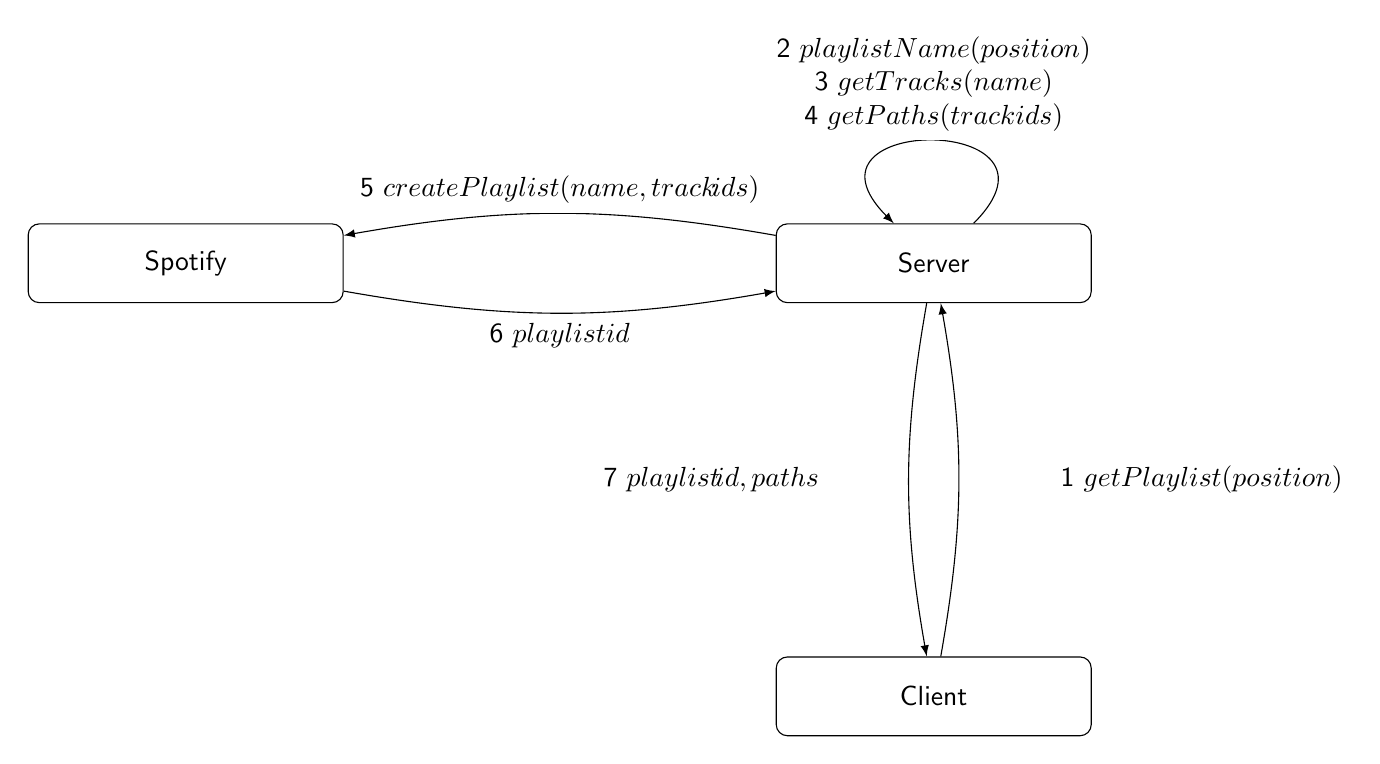
\begin{tikzpicture}[node distance=1.5cm,
    every node/.style={fill=white, font=\sffamily}, align=center]
  % Specification of nodes (position, etc.)

  \node (server)       [base,]                         {Server};
  %\node (database)     [base,above of=server, yshift=4cm]        {Database};
  \node (spotify)      [base,left of=server, xshift=-8cm]        {Spotify};
  \node (client)       [base,below of=server, yshift=-4cm]                   {Client};

\draw[-latex] (client) to[bend right=10] node[left,xshift=5cm] {\circled{1} $getPlaylist(position)$} (server);
\draw[-latex] (server) edge [looseness=5] node[above] {\circled{2} $playlistName(position)$ \\ \circled{3} $getTracks(name)$ \\ \circled{4} $getPaths(trackids)$} (server);

\draw[-latex] (server) to[bend right=10] node[above] {\circled{5} $createPlaylist(name,track\! ids)$} (spotify);
\draw[-latex] (spotify) to[bend right=10] node[below] {\circled{6} $playlistid$} (server);
\draw[-latex] (server) to[bend right=10] node[right,xshift=-4cm] {\circled{7} $playlist \!id,paths$} (client);

\end{tikzpicture}

\subsubsection{Nearest POIs selection algorithm}
Once the client position is validated, it is necessary to select the POIs that will be used for the recommendation.
The recommendation is performed in the following way: select the nearest POI and two other POIs in a range of 2 km, then calculate repartition weights using the following equation:
$$w_i = \Bigg \lfloor 10 \dfrac{\dfrac{1}{\log_2 (d_i + 10)}}{\sum \dfrac{1}{\log_2 (d_i + 10)} } \Bigg \rceil$$

In this way we obtain normalized weights from 0 to 10 that are inversely proportional to the log base 2 of the distance.

\subsubsection{Artist' tracks selection algorithm}
In order to understand the link between the recommended tracks and the POIs, we need to go deeper in the process that links a POI with his tracks.
For each artist there is a direct mapping with its tracks.
The problem is: given a group of POIs, find the correct tracks.
The playlist name encodes the weights of each poi, and each weight express exactly the number of tracks that must be chosen for the POI associated.
Since each POI is linked to different artists, we need a way to select songs from them in a balanced way.
What we do is to cycle between all the artists to take each time the most important song that is not already present in the playlist. In this way we obtain different songs from different artists, and since the artist and songs are static, the tracks in the playlist will be always the same. In the future we think to add randomization to the whole selection process.

\subsubsection{Response generation}
\begin{enumerate}
\item Create a playlist with the generated playlist name if it does not exist and add previously selected tracks.
\item Attach to each track the path between the poi and the track's artist.
\item Return the playlist ID and the track-path mappings as a JSON.
\end{enumerate}


\section{Mobile Web Application}
\begin{figure}[!htb]
\begin{minipage}[t]{0.45\textwidth}
\includegraphics[width=\linewidth]{images/Player.png}
\caption{Music Player}
\label{fig:music_player}
\end{minipage}
\hspace{\fill}
\begin{minipage}[t]{0.45\textwidth}
\includegraphics[width=\linewidth]{images/Map.png}
\caption{Map}
\label{fig:map}
\end{minipage}

\vspace*{0.5cm} % (or whatever vertical separation you prefer)
\begin{minipage}[t]{0.45\textwidth}
\includegraphics[width=\linewidth]{images/Visualization_1.png}
\caption{Visualization Options}
\label{fig:visualization_option}
\end{minipage}
\hspace{\fill}
\begin{minipage}[t]{0.45\textwidth}
\includegraphics[width=\linewidth]{images/Visualization_2.png}
\caption{Visualization}
\label{fig:visualization}
\end{minipage}

\end{figure}
The Web application is implemented using AngularJS and its common MVC model. Using the Angular framework we are able to create complex single page applications that reduces to the minimum the client server interactions. Another advantage of AngularJS is his widespread adoption and the presence of numerous libraries that communicates naturally with it. One of those is the Google Map module that we use to handle all the POI navigation. In fact all the applications is based on the user position.
The app is composed of three views: Music Player, Map, Relation Visualization.

\subsection{Music Player}
The music player is implemented using the Spotify Play Button. This is a special \textless{}iframe\textgreater that loads a simplified Spotify player for a specified playlist. This solution is extremely convenient because it simply needs a playlist ID to run. Since the playlists are created server side and are recovered using the REST API, the whole process is very simple.
Unfortunately it is not possible to manipulate programmatically the \textless{}iframe\textgreater and this limit the whole user experience. As an improvement, we could build a custom player that still uses the Spotify API.
The list of songs proposed in the player are the ones associated to the artist linked with the POIs nearer to the user.
The player page is visible in Figure \ref{fig:music_player}.

\subsection{Angular Google Maps API}
The Angular Google Maps directive supports the majority of the style attributes that the native API supports. Google’s native web API is used for visualizing maps and accessing rich mapping features. The ones used in the application are:

\begin{enumerate}
\item Markers: they are used to identify the POIs and the user position on the map
\item Directions: they are used to give directions that allow the user to reach easily a specific POI on the map.
\end{enumerate}

The map view is composed of two elements: the big navigation map and on the bottom a small Spotify player. Figure \ref{fig:map})

\subsection{Relation visualization}
This view allows the user to visualize the link between POIs and artists. This is essential to deeply understand why a specific artist is recommended for a specific POI. Moreover, one of the goals of the project is to stimulate the user curiosity, proposing interesting connections between music and places.
In order to draw the connection graph we use 'Sigma.js`'\footnote{Sigma.js: http://sigmajs.org/}, a JavaScript library dedicated to graph drawing. For our application the library is useful for the following purposes:
\begin{enumerate}
\item It offers a pretty good path visualization.
\item It can define labels and styles to attach to nodes and edges.
\item It allows to open a window associated with nodes and edges by clicking on them. The window shows the page related to the resource in the graph.
\end{enumerate}
In order to start visualizing connections it is necessary to select a composer between the ones linked with the songs in the playlist and a POI between the ones kept into consideration for the recommendation (Figure \ref{fig:visualization_option}).

After selecting these options is possible to see the path between selected POI and the selected artist. This is showed in the Figure \ref{fig:visualization}. The green node represents the song related to the artist, the artist node is red, the POI node is blue. The middle resource that links POI and artist is represented in yellow.

\section{Conclusion and Future Work}
In this work, we presented CityMusic: a context-aware content-based recommender system for artists.
Regarding the first part: the interlinking, we showed that is possible to link POIs and artists to DBpedia achieving good metrics by using only the POI labels. In addition we linked also the Doremus artists with both Dbpedia and Wikidata artists, with an high level of precision. The quality allowed to correct some ISNI mistakes and to propose matchings that are not present in ISNI in order to add them to Doremus.

We worked on the Relfinder algorithm, by making it scalable. Having a scalable solution for the relation finding is crucial for any project that aims to use heavily the huge knowledge graph that DBpedia contains. So we developed a solution that is computationally efficient and that can be executed in short times. This allowed us to explore the semantic graph with high depths, retrieving a big number of paths.

We proposed a metric to select the best paths between the ones retrieved. This metric drove to discover some particular paths, as the one linked to Yannick Noah.

Our future plans are:
\begin{enumerate}
\item Improve the relation finding algorithm allowing it to find more complex relations without affecting performances. In the case of the artist for example, we should try to increase the number of matchings considering the linked works.
\item Improve the relation selection algorithm: this part needs a big rework because in the selected paths, there are some that are not meaningful for the user. In addition we should try to explore the semantic graph not considering only one middle path but all possible. Actually we develop an algorithm that perform this job, but it's difficult to control the number of entities retrieved by the queries.
\item Evaluate the overall approach with real users.
\item Use additional context information available in 3cixty and DOREMUS. In this optic, 3cixty provides information about events and this could be added in the recommendation engine, maybe suggesting songs or artists that will be played in a place in the near future.
\item Integrate the music context in the recommendation: now we recommend popular songs because we are not able to choose among them based on the current context. By linking DOREMUS songs with DBpedia we hope to extend the semantic recommendation taking into account song-specific relations with a POI. Linking songs to DBpedia is hard, but we showed that is possible. The main challenge continue to be the search for good relations between POIs and Songs. This operation is even harder than linking artists to POIs because songs on DBpedia are very poorly described, and have big lacks in links with other resources.
\end{enumerate}
\bibliographystyle{unsrt}
\bibliography{report}
\end{document}
